\documentclass[a4paper,twocolumn,11pt,twoside]{article}

\usepackage[utf8]{inputenc}
\usepackage[T1]{fontenc}
\usepackage{amsmath}
\usepackage[adobe-utopia]{mathdesign}
\usepackage{microtype}

\usepackage[italian]{babel}
\usepackage{indentfirst}

\usepackage{lipsum}

\usepackage{tikz}

\title{Relazione finale laboratorio di Fisica Computazionale}
\author{Jordi Fabris, Andrea Lanterna}
\date{}

\begin{document}

\maketitle

\section{La discretizzazione di problemi a una dimensione}
Affrontare numericamente problemi di meccanica quantistica rende possibile trovare soluzioni non determinabili analiticamente, ovvero la larghissima maggioranza dei problemi, ma implica l'insorgere di una serie di complicazioni dovute al fatto che le macchine reali siano incapaci di lavorare direttamente con insiemi infiniti.

\begin{equation}
    \begin{cases}
        \hat{H}\psi &=\lambda\psi \\
        \hat{H} &=\hat{H}_0+V \\
        \hat{H}_0 &=-\frac{\hbar}{2m} \frac{d^2}{dx^2}
    \end{cases}
    \rightarrow
    \begin{cases}
        H\psi_n &=\lambda_n\psi_n \\
        H &=H_0+V \\
        H_0 &=-\frac{d^2}{2dx^2}
    \end{cases}
    \label{hsys}
\end{equation}

Per ridurre il problema a una formulazione discreta è ridurre la cardinalità da continua a finita, passando dalla retta reale a un reticolo limitato di \(N\) punti di passo \(a\) come illustrato in Fig. \ref{1Dlattice}: così facendo il problema è definito su un grafo e può essere affrontato con gli strumenti matematici propri di questa struttura, tra i quali spiccano le matrici. 

\begin{figure}
    \centering
    \begin{tikzpicture}
        \draw[thick,dashed] (0,0) -- (0.5,0) node[anchor=north west] {};
        \draw[thick,->] (0.5,0) -- (5,0) node[anchor=north west] {$\mathbb{R}$};
        \foreach \x in {1,2,3,4}
            \draw (\x cm,3pt) -- (\x cm,-3pt) node[anchor=north] {};
        \foreach \x in {1.5,2.5,3.5}
            \filldraw (\x cm,0) circle (2pt);
    \end{tikzpicture}
    \caption{Reticolo monodimensionale sovraimposto alla retta reale}
    \label{1Dlattice}
\end{figure}

Sotto queste condizioni infatti \(\hat{H}\) in (\ref{hsys}) è degradato da operatore a matrice quadrata finita, rendendo il problema affrontabile numericamente. Per farlo è utile spostarsi nelle unità naturali del problema: definendo \( \frac{\hbar^2}{m} = 1\) la forma in cui è comodo scrivere il problema è riportata in (\ref{numver}). In questo modo è facile distinguere l'operatore cinetico dal potenziale generico e distinguere possibili linee d'intervento per l'implementazione delle soluzioni numeriche. 

\begin{equation}
    \Bigg[-\frac{d^2}{2dx^2}+V(x)\Bigg]\psi=E\psi
    \label{numver}
\end{equation}

\subsection{Rappresentazioni discrete dell'operatore cinetico \(H_0\)}

Dalla (\ref{numver}) si vede chiaramente come l'operatore cinetico\(H_0\) sia un laplaciano discreto \(\Delta\) a meno di una costante moltiplicativa. La costruzione di questa matrice può essere ottenuta in due modi principali: come sviluppo di Taylor o  sfruttando la diagonalità di \(H_0\) nello spazio dei momenti coniugati tramite la trasformata di Fourier. Pregi e difetti di entrambi gli approcci verranno discussi nelle prossime sezioni 

\subsubsection{L'operatore cinetico come sviluppo di Taylor}

L'equazione (\ref{numver}) intesa su un grafo evidenzia come \(H_0\) debba agire come matrice quadrata: sviluppando una funzione di test \(\psi\) nell'intorno di un punto \(x\) del reticolo si ottiene
\begin{equation}
    \begin{aligned}
    \psi(x\pm a)&=\psi(x)\pm a\psi'(x) \\
                &+ \frac{1}{2}a^2\psi''(x) \\
                &+ \dots + o(a^n) \\
    \end{aligned}
\end{equation}

e, a seconda del termine in cui si decide di arrestare lo sviluppo, un'approssimazione progressivamente migliore. Nel caso ci si fermi al secondo ordine la matrice dell'operatore cinetico assume la forma
\begin{equation}
    (\Delta\psi)_j \simeq -\frac{1}{a^2}(\psi_{j+1}-2\psi_j+\psi_{j-1})
\end{equation}

L'approssimazione di ordine arbitrario indicata come
\begin{equation}
    \begin{aligned}
    \alpha_0\psi(x) &= \alpha_1[\psi(x+a)+\psi(x-a)]+ \\
                    &+ \alpha_2[\psi(x+2a)+\psi(x-2a)]+ \\
                    &+ \dots + \alpha_n[\psi(x+na)+\psi(x-na)] \\
    \end{aligned}
\end{equation}
assume la forma generica 
\begin{align}
    (\Delta\psi)_j \simeq
    \frac{1}{a^2} \sum_{k=-n}^{n}\bigg(\alpha_{|k|}\psi_{j+k}\bigg)
\end{align}
con \(\alpha\) definito come soluzione del sistema lineare \(A\alpha = b\), dove
\begin{equation}
    A=
    \begin{pmatrix}
    1 & 2   & 2   & \cdots & 2   \\
    0 & 2^2 & 3^2 & \cdots & k^2 \\
    0 & 2^4 & \ddots & \ddots  \\
    \vdots & \vdots & \ddots & \ddots  \\
    0 & 2^{2(j-1)} &  &  & k^{2(j-1)} \\
    \end{pmatrix}; \quad
    b=
    \begin{pmatrix}
    0 \\
    1 \\
    0 \\
    \vdots \\
    0 \\
    \end{pmatrix}
    \label{Asys}
\end{equation}

\subsubsection{L'operatore cinetico come trasformata di Fourier}

Un approccio più sofisticato al problema sfrutta il fatto che \(H\) sia diagonale nello spazio dei momenti \(k\), legato allo spazio delle posizione \(x\) da una trasformata di Fourier.
Avendo a disposizione degli algoritmi sofisticati, come la FFT, per la trasformazione di Fourier diretta e inversa, è possibile rappresentare H nello spazio delle posizioni come la trasformata inversa del prodotto nello spazio dei momenti della trasformata dall'identità per la rappresentazione diagonale di H. Questo approccio ha il vantaggio di essere molto più rapido del metodo che sfrutta lo sviluppo di Taylor di ordine superiori.

\subsubsection{Le condizioni al contorno}

Le matrici così costruite considerano il problema definito su un grafo illimitato, a differenza di quello su cui è opportuno definirlo, che è di lunghezza finita: per compiere questo ultimo passaggio è necessario capire come imporre le condizioni al contorno al problema modificando opportunamente la matrice \(H\). 

Le condizioni al contorno possibili sono due: le condizione al contorno periodiche o quelle di Dirichlet. Per risolvere il problema è particolarmente utile ragionare sul grafo: per rendere il grafo periodico è necessario collegare i due estremi aperti del reticolo tra loro, imponendo \(\psi_j=\psi_{j+N}\).
Per applicare le condizioni di Dirichlet invece si collegano i due estremi aperti a loro stessi, o a dei punti "virtuali" che impongano \(\psi_0=\psi_{N+1}=0\).

All'atto pratico l'implementazione delle condizioni al contorno si concretizza in modi diversi a seconda del metodo di costruzione.

\paragraph{Le condizioni al contorno nella matrice n-diagonale}
Con il metodo di costruzione n-diagonale si può interpretare \(H\) come una sorta di matrice di adiacenza del grafo: in questo caso le condizioni Dirichlet vengono imposte ponendo uguali a zero gli opportuni vertici, o imponendo una struttura "ad anello", ovvero negli stessi vertici posti a zero si impongo valori tali che si possa ripetere la matrice stanti delle permutazioni di righe.

\paragraph{Le condizioni al contorno nella matrice di Fourier}
Con il metodo di costruzione che sfrutta la trasformata di Fourier è impossibile procedere direttamente come illustrato sopra data la doppia trasformazione. Metodo ifft sinft.

\subsection{Valutazione quantitativa su problemi con potenziale armonico}

Si procede alla valutazione dell'efficienza e dell'efficacia di questi metodi comparando i risultati nella ricerca degli autovalori di un problema con potenziale di tipo armonico, di forma \(V=\frac{1}{2}\omega^2 x^2\), usando come parametri di valutazione la precisione rispetto alle soluzioni analitiche e il tempo d'esecuzione. 

L'implementazione di entrambi i metodi è affidata a \verb|harmtest.m|, che si basa su chiamate multiple di \verb|makeh.m|, cui è affidata l'implementazione degli algoritmi, al variare di un singolo parametro, ovvero \verb|lap_approx|, che determina il metodo di costruzione della matrice H. Nella convenzione scelta nel caso questo valore sia 0 verrà costruita tramite trasformazione di Fourier, altrimenti per valori maggiori \verb|lap_approx| rappresenta la dimensione del vettore \(\alpha\) come definito in (\ref{Asys}), legata al numero di diagonali dalla relazione \(n_d=(2 \cdot \dim(\alpha)-1)\).

\begin{figure}
    \centering
    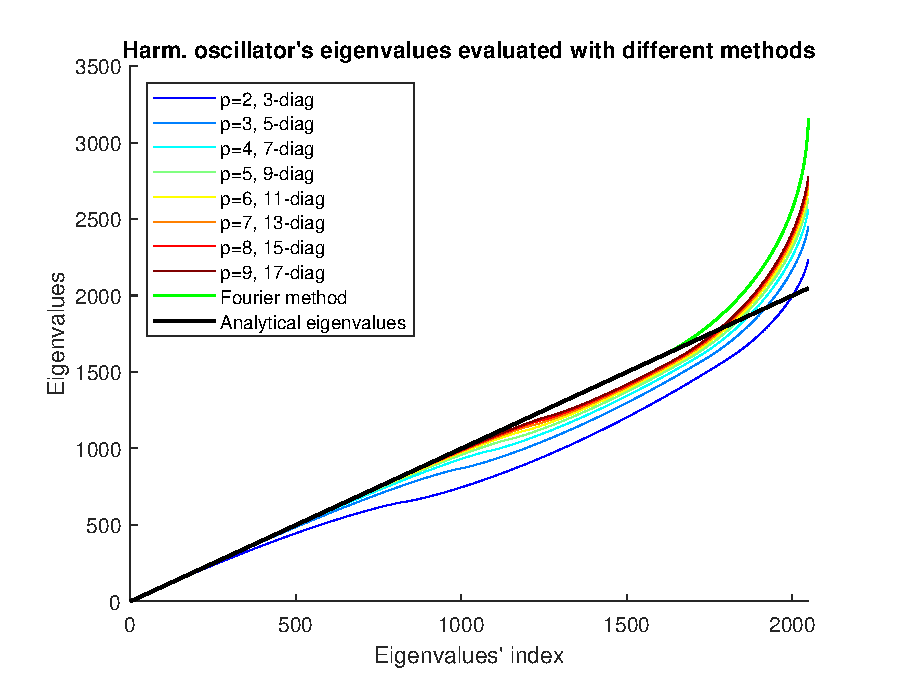
\includegraphics[width=1.0\columnwidth]{heig}
    \caption{Confronto tra i diversi metodi di calcolo degli autovalori}
    \label{heig}
\end{figure}

\begin{figure}
    \centering
    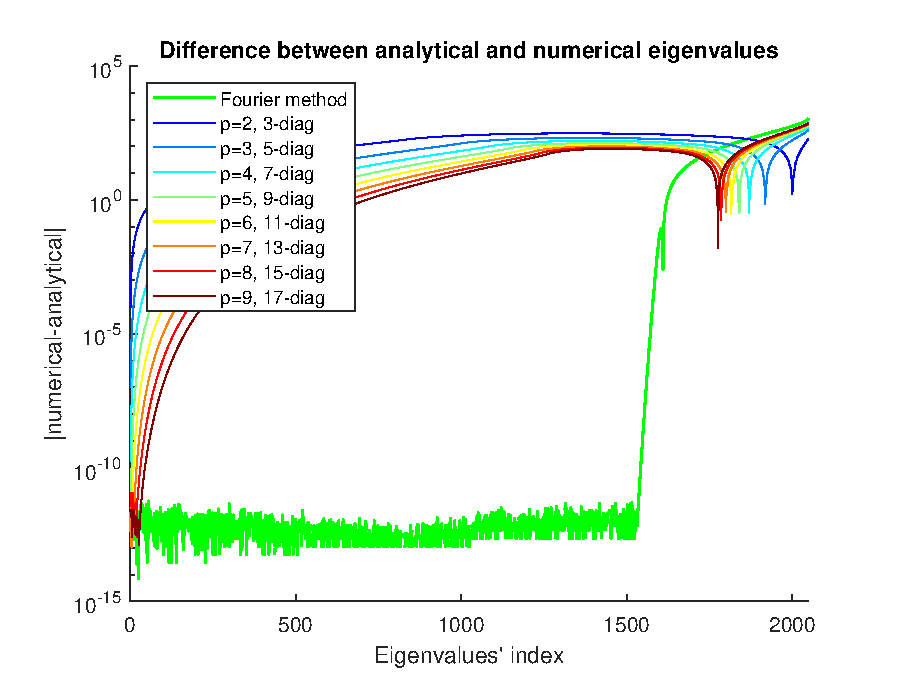
\includegraphics[width=1.0\columnwidth]{deig}
    \caption{Differenza tra autovalori analitici e autovalori numerici}
    \label{deig}
\end{figure}

In Fig. \ref{deig} è ben evidenziato come l'algoritmo che sfrutta la trasformata di Fourier abbia enormi vantaggi dal punto di vista della precisione rispetto a qualsiasi variante del metodo n-diagonale, che non è in grado di produrre, nell'implementazione proposta, approssimazioni per valore di \(p>9\) in quanto incapace di risolvere (\ref{Asys}) per matrici di tali dimensioni.

\begin{figure}
    \centering
    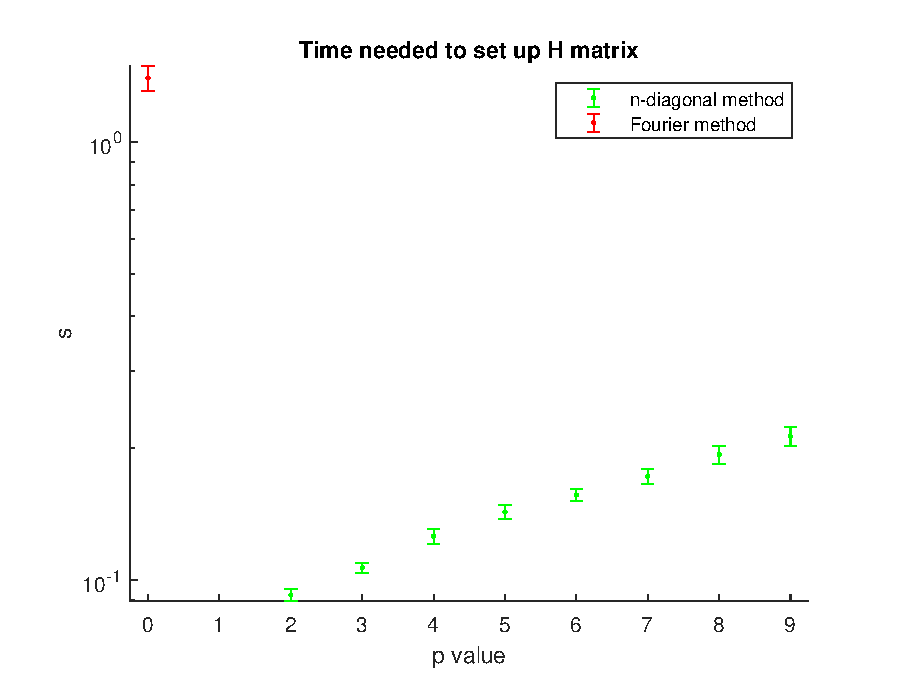
\includegraphics[width=1.0\columnwidth]{teig}
    \caption{Tempo medio per la valutazione della matrice H}
    \label{teig}
\end{figure}

In Fig. \ref{teig} è mostrato il costo computazionale valutato come tempo medio d'esecuzione su 15 tentativi dei vari metodi: il metodo di Fourier è un'ordine di grandezza più lento del peggior caso possibile del metodo n-diagonale, ma l'enorme vantaggio in termini di precisione, che raggiunge anche i dieci ordini di grandezza, giustifica la differenza.

\section{Un caso di studio: il potenziale \(|x|^\alpha\)}
Un problema di particolare interesse fisico è 
\begin{equation*}
    H=-\frac{\hbar^2}{2m}\frac{d^2}{dx^2}+\frac{1}{2}g|x|^\alpha
\end{equation*}
che, in opportune unità di misura può essere scritto come
\begin{equation}
    H=-\frac{d^2}{2dx^2}+\frac{1}{2}|x|^{\alpha}
\end{equation}

Prenderemo in analisi una famiglia di problemi con \(\alpha>0\) con particolare attenzione ai casi in cui \(\alpha \neq 2\) per il quali non è disponibile una soluzione analitica ma solo la formula di quantizzazione semiclassica di Bohr-Sommerfeld, che impone valori quantizzati dell'azione ridotta
\begin{equation}
    I = \oint pdx = 2\pi\hbar\bigg(n+\frac{1}{2}\bigg), \quad n=0,1,2,\dots
    \label{borsom}
\end{equation}

Fissando un valore d'energia \(E\) si identifica, data la simmetria del potenziale, un intorno di 0 di raggio \(x_0\). Da questo fatto si può, sfruttando la conservazione l'energia, derivare \(E=\frac{1}{2}|x|^\alpha\). Dato che \(p=\sqrt{2E-|x|^\alpha}\), ridefinendo \(\lambda = \frac{x}{x_0}\) si può riscrivere la (\ref{borsom}) come 
\begin{equation}
    I = 4x^{1+\frac{\alpha}{2}}_0\int_0^1\sqrt{1-\lambda^\alpha}d\lambda
\end{equation}

L'integrale (\ref{borsom}) è affrontabile numericamente, restituendo come risultato un integrale di Eulero di secondo tipo, o Gamma di Eulero

\begin{equation}
    I = 4x^{1+\frac{\alpha}{2}}_0\frac{\beta\big(\frac{3}{2},\frac{1}{\alpha}\big)}{\alpha}
\end{equation}

L'espressione per le energie semiclassiche è quindi

\begin{align*}
    E_n & =
    \frac{1}{2}\Bigg(\frac{\pi\alpha}{2\beta\big(\frac{3}{2},\frac{1}{\alpha}\big)}\Bigg)^\frac{2\alpha}{\alpha+2} &\Bigg(n+\frac{1}{2}\Bigg)^\frac{2\alpha}{\alpha+2} \\
    :&= c_{\alpha} &\Bigg(n+\frac{1}{2}\Bigg)^\frac{2\alpha}{\alpha+2} \\
    n&=1,2,\dots\\
\end{align*}

Dalla formula semiclassica è facile vedere come per \(\alpha=2\) i valori coincidano con gli autovalori del sistema calcolati per via analitica e già usati come termine di paragone in precedenza.

\section{L'equazione di Schroedinger dipendente dal tempo}
\begin{equation}
    \dot{\psi}=-iH\psi
\end{equation}
Esistono diversi approcci per la soluzione numerica dell'equazione di Schroedinger dipendente dal tempo ma in generale gli approcci possono essere catalogati in due categorie principali: i metodi che si basano sulla risoluzione dell sistema di equazioni a derivate parziali e i metodi che si basano sul calcolo di una matrice \(U\) tale che \(\psi(t)=U\psi(0)\).

Di seguito verranno studiati tre approcci: uno del primo tipo, che si basa sulla riduzione del problema alle derivate parziali, e due del secondo, usando alternativamente un algoritmo simplettico o il calcolo di esponenziale di matrice.

\subsection{Soluzione tramite equazione differenziale ordinaria}

\subsection{Soluzione tramite esponenziale di matrici}

\subsection{Soluzione tramite algoritmo simplettico}

\section{Un caso di studio: il potenziale \(pinco pallino\)}
Delte finte e polinomi
\end{document}